\subsubsection{The Response Matrix}
\label{subsection: charged particle event multiplicity, the response matrix}

The efficiency correction for the multiplicity distribution is modelled by the response matrix $R$. This characterises the effect of the detector response on the charged particle multiplicity distribution, it is a two dimensional matrix with dimensions of $n$ by $m$ where each element $R_{ij}$, corresponds to the probability to reconstruct $i$ tracks given that $j$ prompt particles are present in the event (constraining the values along the columns so that their sum is normalised to one). The relationship between the track multiplicity $a$, true multiplicity $b$ and response matrix $R$ can be then expressed as a matrix equation,

%The multiplicity correction uses the response matrix as discussed. The relationship between the reconstructed distribution, true distribution and detector response is given by,

\begin{equation}
	\label{equation: multiplicity-response relationship}
	a = R \cdot b
\end{equation}

where a and b are column matrices describing the track and particle multiplicities such that $a_i$ is the number of events with $i$ reconstructed tracks and $b_j$ is the number of events with $j$ corresponding true particles. This can be interpreted as a set of linear equations,

\begin{equation}
	a_i = \sum_{j=0}^m{R_{ij} \cdot b_j} \,\,\,\,\,\,\,\,\,\,\,\,\,\,\,\,\,\,\,\, i \in \{0, 1, ... , n\}
\end{equation}

%Hence the true distribution, $b$ is given by,
%
%\begin{equation}
%	b = R^{-1} \cdot a
%\end{equation} 
%
%where $R^{-1}$ is the inverse of the response matrix, $R$. The inversion of the response matrix is not a trivial task, instead a more heuristic approach is used. 
%
%where a and b are column matrices describing the track and particle multiplicities respectively such that $a_i$ is the number of events with $i$ reconstructed tracks and $b_j$ is the number of events with $j$ corresponding true particles.

\begin{figure}
	\centering
	\begin{subfigure}{0.32\textwidth}
		\includegraphics[width=\textwidth]{/afs/cern.ch/user/d/dvoong/cmtuser/DaVinci_v33r6/Phys/ChargedParticleMultiplicity/python/response_matrix/data_files/ResponseMatrixPlottingJob/bk/Down/mc/-1/-1/bk/Down/mc/-1/-1/meissner_multiplicity_full/bk/Down/mc/-1/-1/bk/Down/mc/-1/-1/background_corrected/pngs/2_0-4_5.png}
		\caption{$2.0 \le \eta \le 4.5$}
	\end{subfigure}
	\begin{subfigure}{0.32\textwidth}
		\includegraphics[width=\textwidth]{/afs/cern.ch/user/d/dvoong/cmtuser/DaVinci_v33r6/Phys/ChargedParticleMultiplicity/python/response_matrix/data_files/ResponseMatrixPlottingJob/bk/Down/mc/-1/-1/bk/Down/mc/-1/-1/meissner_multiplicity/bk/Down/mc/-1/-1/bk/Down/mc/-1/-1/background_corrected/pngs/2_0-2_5.png}
		\caption{$2.0 \le \eta \le 2.5$}
	\end{subfigure}
	\begin{subfigure}{0.32\textwidth}
		\includegraphics[width=\textwidth]{/afs/cern.ch/user/d/dvoong/cmtuser/DaVinci_v33r6/Phys/ChargedParticleMultiplicity/python/response_matrix/data_files/ResponseMatrixPlottingJob/bk/Down/mc/-1/-1/bk/Down/mc/-1/-1/meissner_multiplicity/bk/Down/mc/-1/-1/bk/Down/mc/-1/-1/background_corrected/pngs/2_5-3_0.png}`
		\caption{$2.5 \le \eta \le 3.0$}
	\end{subfigure}
	\begin{subfigure}{0.32\textwidth}
		\includegraphics[width=\textwidth]{/afs/cern.ch/user/d/dvoong/cmtuser/DaVinci_v33r6/Phys/ChargedParticleMultiplicity/python/response_matrix/data_files/ResponseMatrixPlottingJob/bk/Down/mc/-1/-1/bk/Down/mc/-1/-1/meissner_multiplicity/bk/Down/mc/-1/-1/bk/Down/mc/-1/-1/background_corrected/pngs/3_0-3_5.png}
		\caption{$3.0 \le \eta \le 3.5$}
	\end{subfigure}
	\begin{subfigure}{0.32\textwidth}
		\includegraphics[width=\textwidth]{/afs/cern.ch/user/d/dvoong/cmtuser/DaVinci_v33r6/Phys/ChargedParticleMultiplicity/python/response_matrix/data_files/ResponseMatrixPlottingJob/bk/Down/mc/-1/-1/bk/Down/mc/-1/-1/meissner_multiplicity/bk/Down/mc/-1/-1/bk/Down/mc/-1/-1/background_corrected/pngs/3_5-4_0.png}
		\caption{$3.5 \le \eta \le 4.0$}
	\end{subfigure}
	\begin{subfigure}{0.32\textwidth}
		\includegraphics[width=\textwidth]{/afs/cern.ch/user/d/dvoong/cmtuser/DaVinci_v33r6/Phys/ChargedParticleMultiplicity/python/response_matrix/data_files/ResponseMatrixPlottingJob/bk/Down/mc/-1/-1/bk/Down/mc/-1/-1/meissner_multiplicity/bk/Down/mc/-1/-1/bk/Down/mc/-1/-1/background_corrected/pngs/4_0-4_5.png}
		\caption{$4.0 \le \eta \le 4.5$}
	\end{subfigure}
	\caption{Response matrices}
	\label{fig: background corrected response matrices}
\end{figure}

The response matrix is determined using truth information from Monte Carlo simulated events. Each event is first subject to the background correction procedure discussed in section \ref{subsection: charged particle multiplicity, background correction} so that the response matrix corresponds only to efficiency effects. As in section \ref{subsection: charged particle multiplicity, background correction} the number of background tracks is varied between its allowed range ($0 \le k \le N$) and the number of signal tracks, $n_\mathrm{signal} = N - k$, is then plotted against the number of prompt particles present in the event, then weighted by the corresponding probability of observing $n_\mathrm{signal}$. Due to insufficient statistics at the high multiplicity regions in the MC data (see figure \ref{fig: background corrected response matrices} the response matrices are truncated to remove elements with low statistical significance, the response matrices calculated for the efficiency correction are shown in figure \ref{fig: truncated response matrices}.

\begin{figure}
	\centering
	\begin{subfigure}{0.32\textwidth}
		\includegraphics[width=\textwidth]{/afs/cern.ch/user/d/dvoong/cmtuser/DaVinci_v33r6/Phys/ChargedParticleMultiplicity/python/response_matrix/data_files/ResponseMatrixPlottingJob/bk/Down/mc/-1/-1/bk/Down/mc/-1/-1/meissner_multiplicity_full/bk/Down/mc/-1/-1/bk/Down/mc/-1/-1/background_corrected/truncation/pngs/2_0-4_5.png}
		\caption{$2.0 \le \eta \le 4.5$}
	\end{subfigure}
	\begin{subfigure}{0.32\textwidth}
		\includegraphics[width=\textwidth]{/afs/cern.ch/user/d/dvoong/cmtuser/DaVinci_v33r6/Phys/ChargedParticleMultiplicity/python/response_matrix/data_files/ResponseMatrixPlottingJob/bk/Down/mc/-1/-1/bk/Down/mc/-1/-1/meissner_multiplicity/bk/Down/mc/-1/-1/bk/Down/mc/-1/-1/background_corrected/truncation/pngs/2_0-2_5.png}
		\caption{$2.0 \le \eta \le 2.5$}
	\end{subfigure}
	\begin{subfigure}{0.32\textwidth}
		\includegraphics[width=\textwidth]{/afs/cern.ch/user/d/dvoong/cmtuser/DaVinci_v33r6/Phys/ChargedParticleMultiplicity/python/response_matrix/data_files/ResponseMatrixPlottingJob/bk/Down/mc/-1/-1/bk/Down/mc/-1/-1/meissner_multiplicity/bk/Down/mc/-1/-1/bk/Down/mc/-1/-1/background_corrected/truncation/pngs/2_5-3_0.png}`
		\caption{$2.5 \le \eta \le 3.0$}
	\end{subfigure}
	\begin{subfigure}{0.32\textwidth}
		\includegraphics[width=\textwidth]{/afs/cern.ch/user/d/dvoong/cmtuser/DaVinci_v33r6/Phys/ChargedParticleMultiplicity/python/response_matrix/data_files/ResponseMatrixPlottingJob/bk/Down/mc/-1/-1/bk/Down/mc/-1/-1/meissner_multiplicity/bk/Down/mc/-1/-1/bk/Down/mc/-1/-1/background_corrected/truncation/pngs/3_0-3_5.png}
		\caption{$3.0 \le \eta \le 3.5$}
	\end{subfigure}
	\begin{subfigure}{0.32\textwidth}
		\includegraphics[width=\textwidth]{/afs/cern.ch/user/d/dvoong/cmtuser/DaVinci_v33r6/Phys/ChargedParticleMultiplicity/python/response_matrix/data_files/ResponseMatrixPlottingJob/bk/Down/mc/-1/-1/bk/Down/mc/-1/-1/meissner_multiplicity/bk/Down/mc/-1/-1/bk/Down/mc/-1/-1/background_corrected/truncation/pngs/3_5-4_0.png}
		\caption{$3.5 \le \eta \le 4.0$}
	\end{subfigure}
	\begin{subfigure}{0.32\textwidth}
		\includegraphics[width=\textwidth]{/afs/cern.ch/user/d/dvoong/cmtuser/DaVinci_v33r6/Phys/ChargedParticleMultiplicity/python/response_matrix/data_files/ResponseMatrixPlottingJob/bk/Down/mc/-1/-1/bk/Down/mc/-1/-1/meissner_multiplicity/bk/Down/mc/-1/-1/bk/Down/mc/-1/-1/background_corrected/truncation/pngs/4_0-4_5.png}
		\caption{$4.0 \le \eta \le 4.5$}
	\end{subfigure}
	\caption{Truncated response matrices}
	\label{fig: truncated response matrices}
\end{figure}